\documentclass[a4paper,10pt]{article}
\usepackage[utf8]{inputenc}
\usepackage{graphicx}
\usepackage{url}
\usepackage{multirow}

%opening
\title{User Guide: Mobile Client Content\\How to Suceed in Sana Without Really Trying}
\author{Sana}

\begin{document}

\maketitle

\begin{abstract}

\end{abstract}

\section{Client User Guide: Try it out}
This guide is for anyone new to the Sana platform and is interested in a quick
demonstration of how it works. 

\subsection{What you should know before you start}
You should have a basic working knowledge of navigating your way through a smart
phone-i.e. how to start an application, menu buttons, back button, etc. Ideally,
you should have tried to install a few apps.

\subsubsection{Hardware and Software}
Nearly any Android based smartphone made after 2010 should work. If you are 
concerned please check your phone manufacturers specs against the following.

\begin{tabular}{ l l }
Hardware&Android phone running 1.6 or later. \\
Software&None but the Sana app.(Instructions for download are below
\end{tabular}

\newpage

\subsection{Mobile Client}
\subsubsection{Downloading}
Installing the client can be performed using your phones scanner or using a url 
for download.

\noindent\begin{tabular}[t]{ c c c }
\parbox{2.1in}{Open a browser. Press or enter the following URL into the location bar:}&\multirow{2}{*}{or}&\parbox{2.1in}{From your phone, scan the following image:} \\
Get Sana!& &\parbox{2.1in}{
\includegraphics{client_install_barcode.png}} \\
\end{tabular}

\begin{center}
Get Sana! = \url{http://moca.googlecode.com/files/sana-release-1.1.apk}
\end{center}
 
\noindent You may also have to browse to your Downloads folder and select the 
sana-release-1.1.apk file.

\subsubsection{Installing}
\noindent Once downloaded, select your downloads notificiations. 

\begin{flushleft}
\begin{tabular}{ c c c c c }
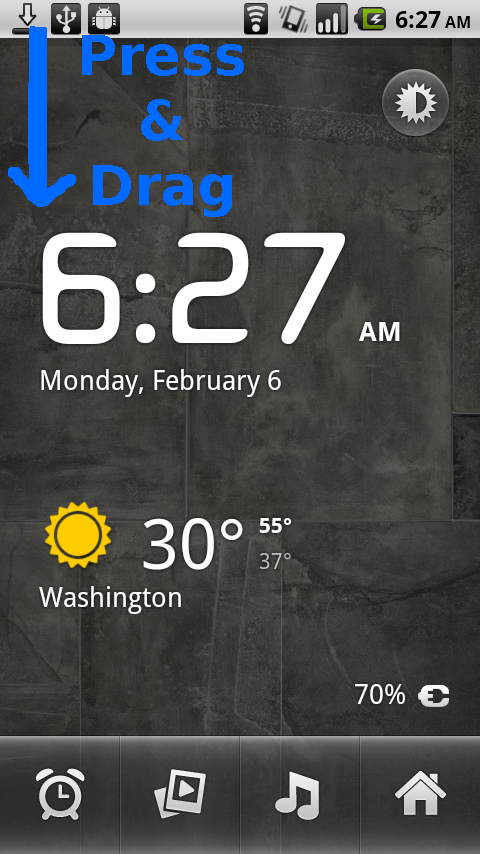
\includegraphics[scale=0.15,keepaspectratio=true]{client_download_notification.png}
&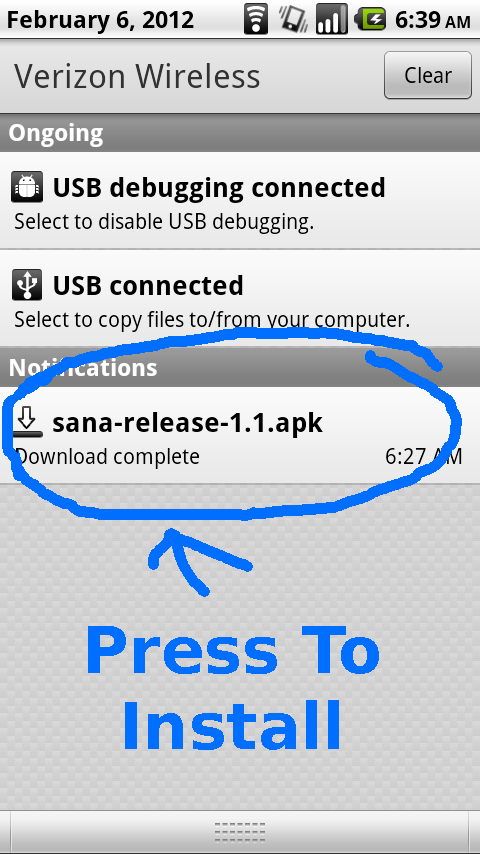
\includegraphics[scale=0.15,keepaspectratio=true]{client_download_notification_expanded.png}
&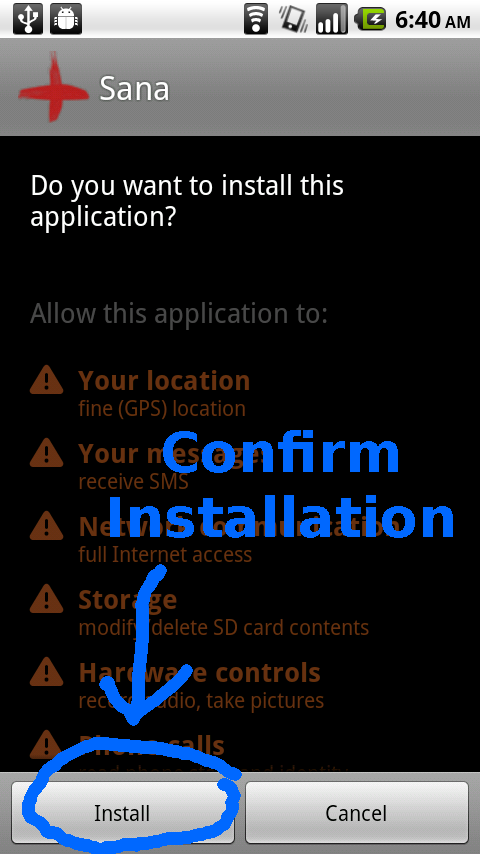
\includegraphics[scale=0.15,keepaspectratio=true]{client_install_confirmation.png}
&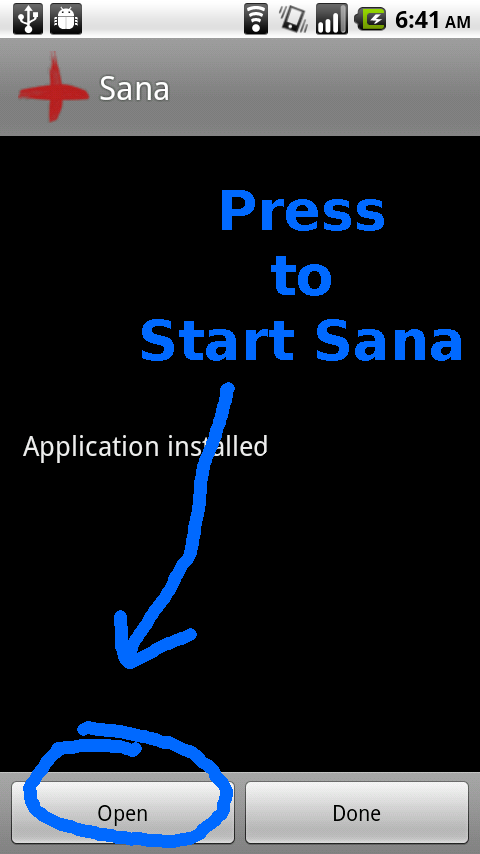
\includegraphics[scale=0.15,keepaspectratio=true]{install_complete.png}
&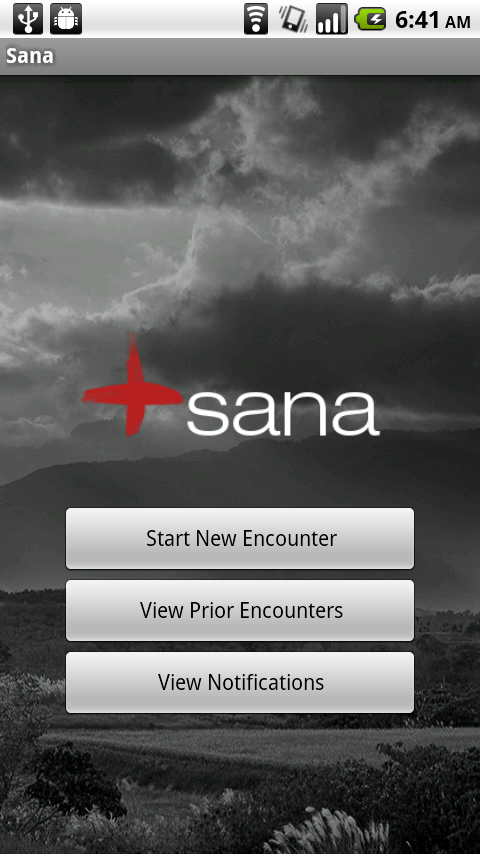
\includegraphics[scale=0.15,keepaspectratio=true]{sana_splash.png}
\end{tabular}
\end{flushleft}

\noindent Once installation is complete, press the back button and the Sana app
should start. 
\newpage

\subsection{Try an App}This section shows a few screenshots from a simple 
procedure which will allow you to collect a few pieces of data and upload them
to the Sana demo server. The application must first have the sample procedures 
loaded. Starting with the main Sana screen visible, press the menu button on 
your phone and walk through the following steps:

\begin{flushleft}
\begin{tabular}{ c c c c }
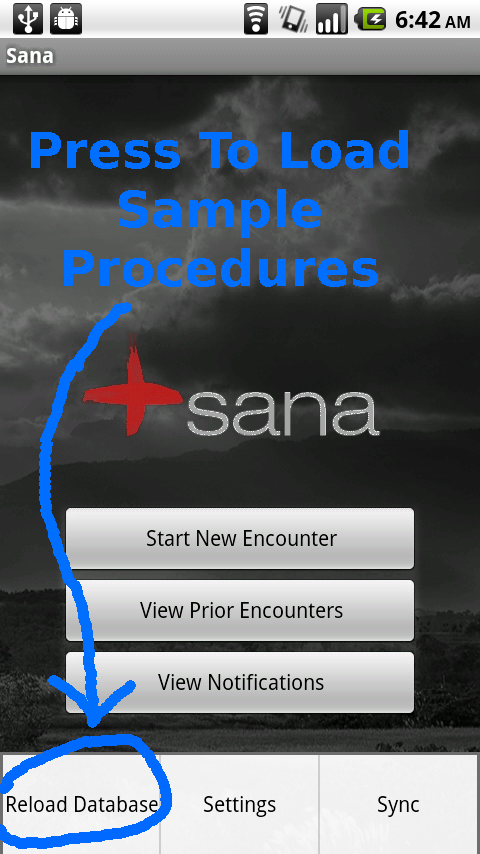
\includegraphics[scale=0.15,keepaspectratio=true]{sana_splash_load_db.png}
&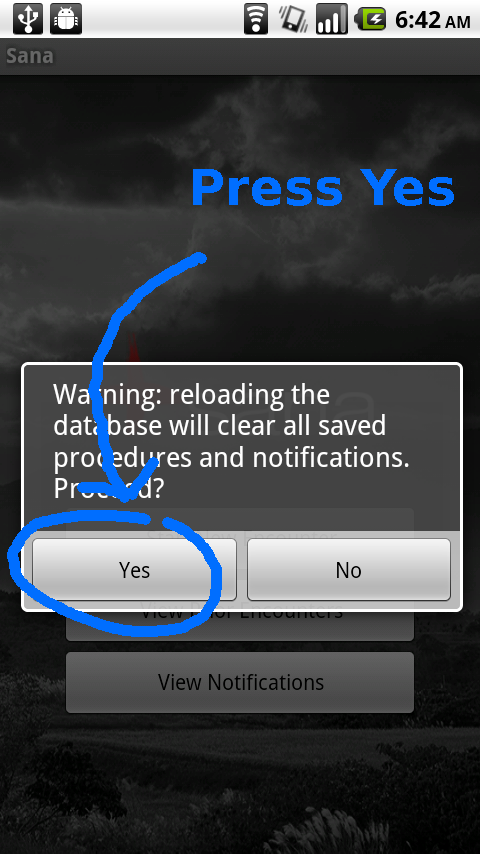
\includegraphics[scale=0.15,keepaspectratio=true]{sana_splash_load_db_confirm.png}
&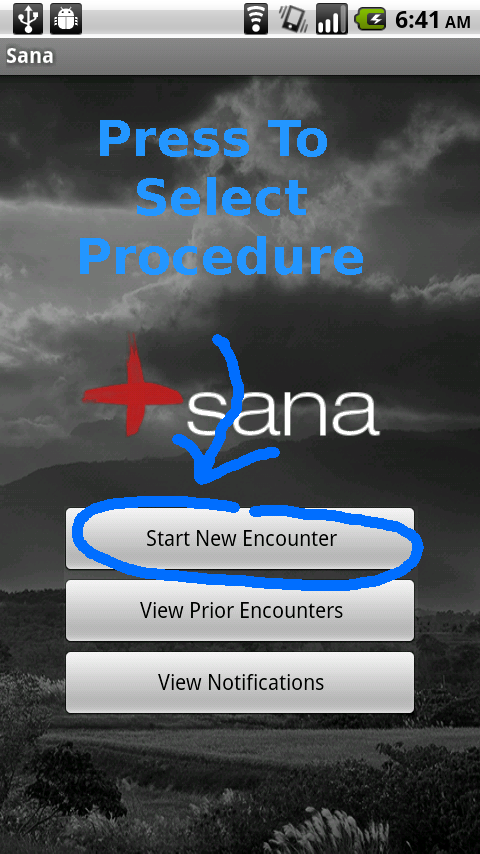
\includegraphics[scale=0.15,keepaspectratio=true]{sana_splash_new_encounter.png}
&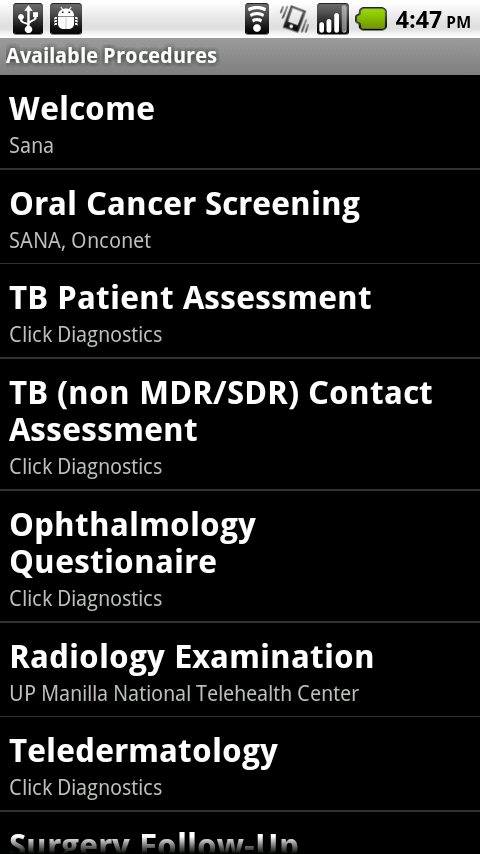
\includegraphics[scale=0.15,keepaspectratio=true]{client_select_procedure.png}
\end{tabular}
\end{flushleft}

\paragraph{Select and Run}Sample exam, very generic
 - Name, Gender, height, weight, age, Family history of cholestoral? Y/N, Have 
you experienced discomfort in your foot in the past week? once, couple times, 
many times, Image of foot

\paragraph{Navigating through a procedure}Navigation through the procedures 
happens with the ``next'' button at the bottom of the screen. The following
images display a small sample of the available steps you will encounter as you
navigate the sample encounters.

\begin{flushleft}
\begin{tabular}{ c c c c }
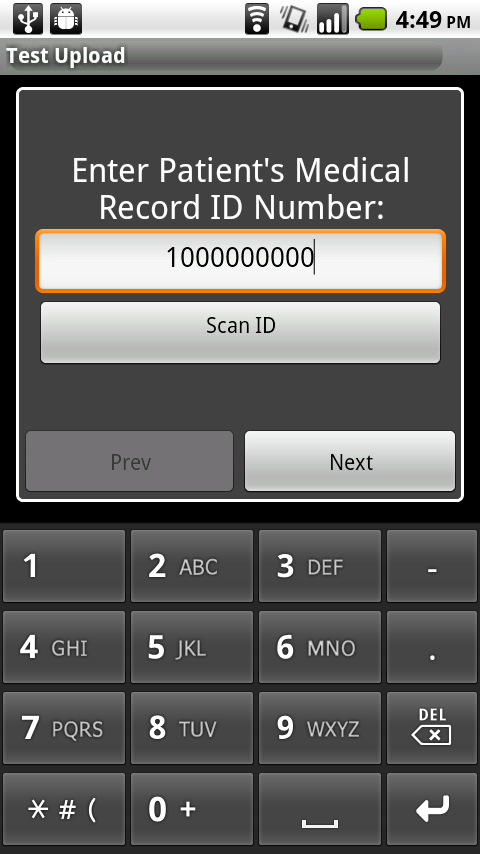
\includegraphics[scale=0.15,keepaspectratio=true]{client_proc_pt_id.png}
&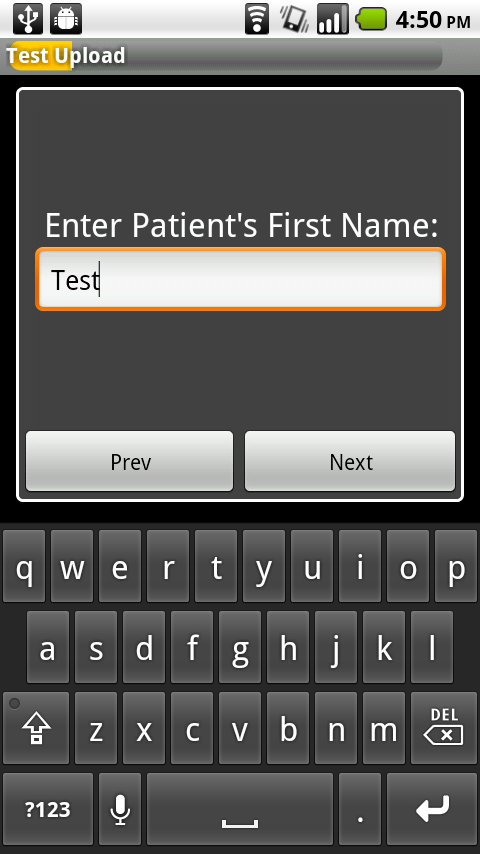
\includegraphics[scale=0.15,keepaspectratio=true]{client_proc_pt_first.png}
&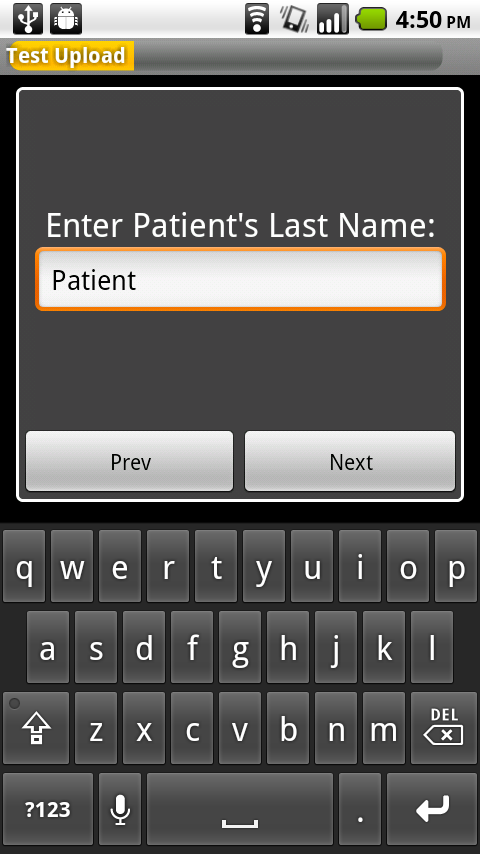
\includegraphics[scale=0.15,keepaspectratio=true]{client_proc_pt_last.png}
&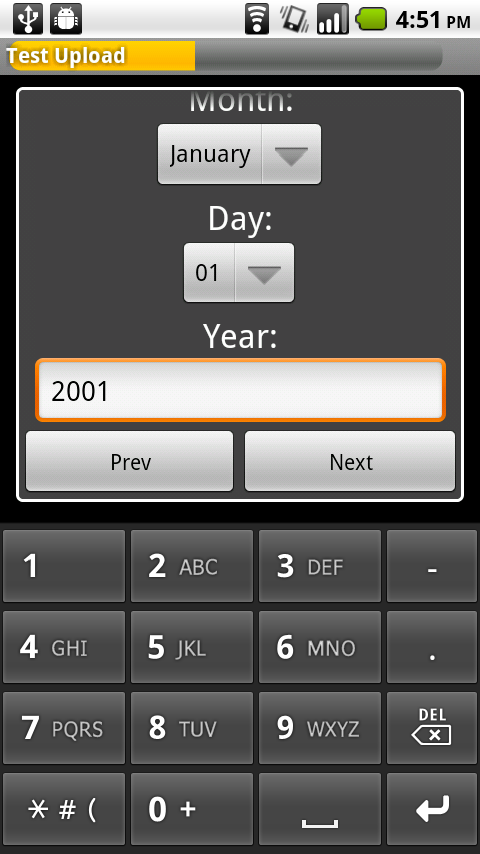
\includegraphics[scale=0.15,keepaspectratio=true]{client_proc_pt_dob.png} \\
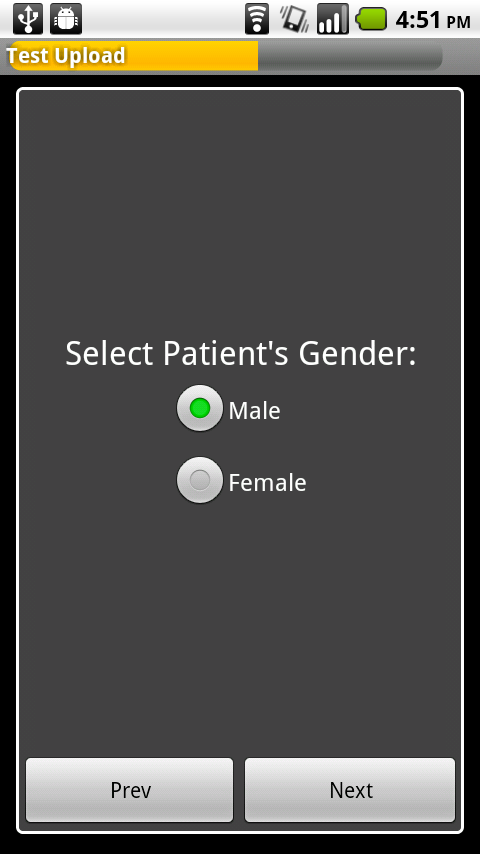
\includegraphics[scale=0.15,keepaspectratio=true]{client_proc_pt_gender.png}
&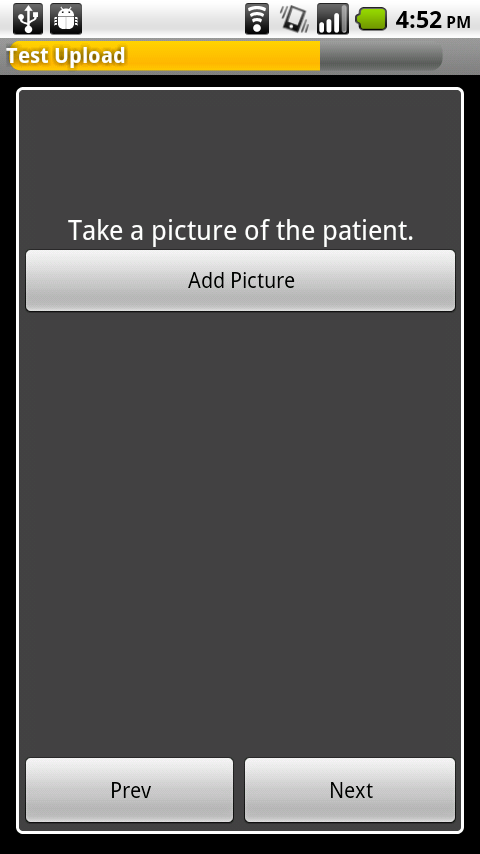
\includegraphics[scale=0.15,keepaspectratio=true]{client_proc_pt_picture.png}
&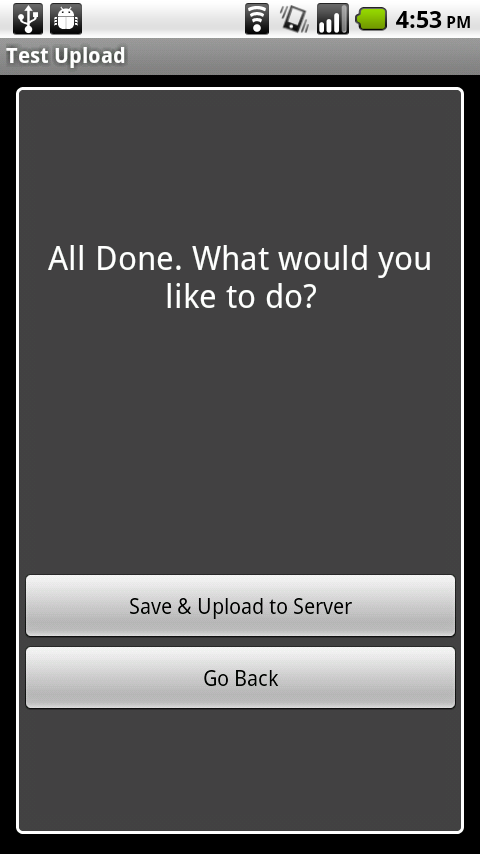
\includegraphics[scale=0.15,keepaspectratio=true]{client_proc_done.png}
&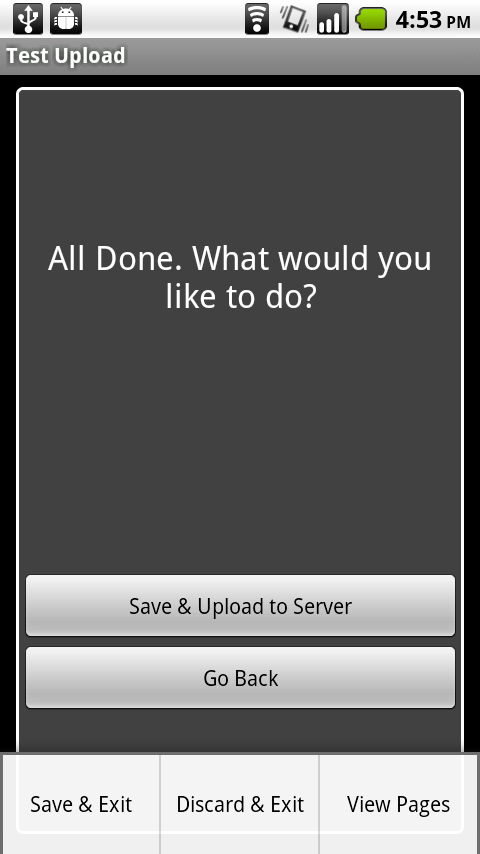
\includegraphics[scale=0.15,keepaspectratio=true]{client_proc_menu.png}
\end{tabular}
\end{flushleft}
\newpage

\subsection{Connect to Database}
The encounter has now been uploaded to a Sana hosted OpenMRS demonstration 
server where you may view your collected data. From your phone or other web 
enabled device, open a browser and enter:

\begin{center}
\url{https://demo.sana.csail.mit.edu/openmrs/index.htm}
\end{center}

\begin{flushleft}
\begin{tabular}{ c c }
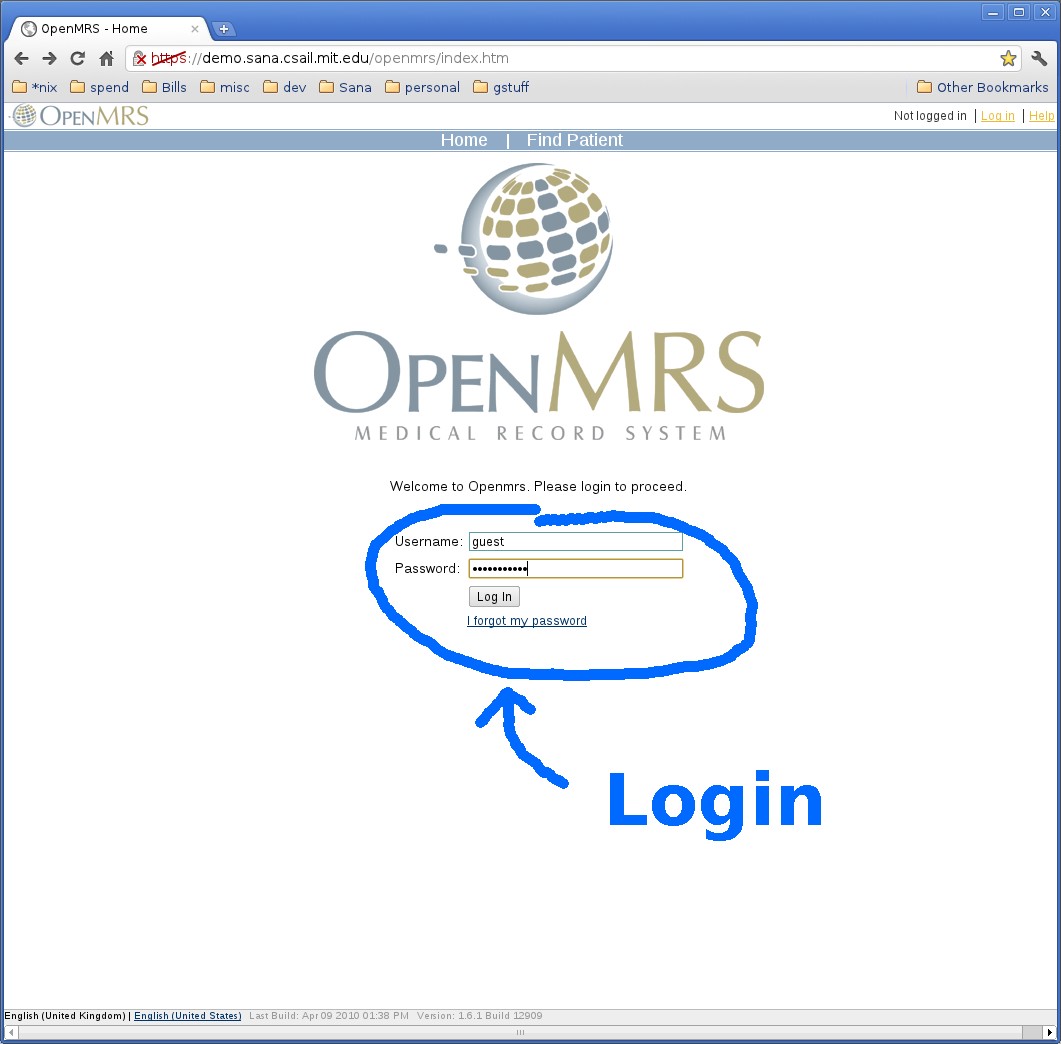
\includegraphics[scale=0.25,keepaspectratio=true]{openmrs_login.png}
&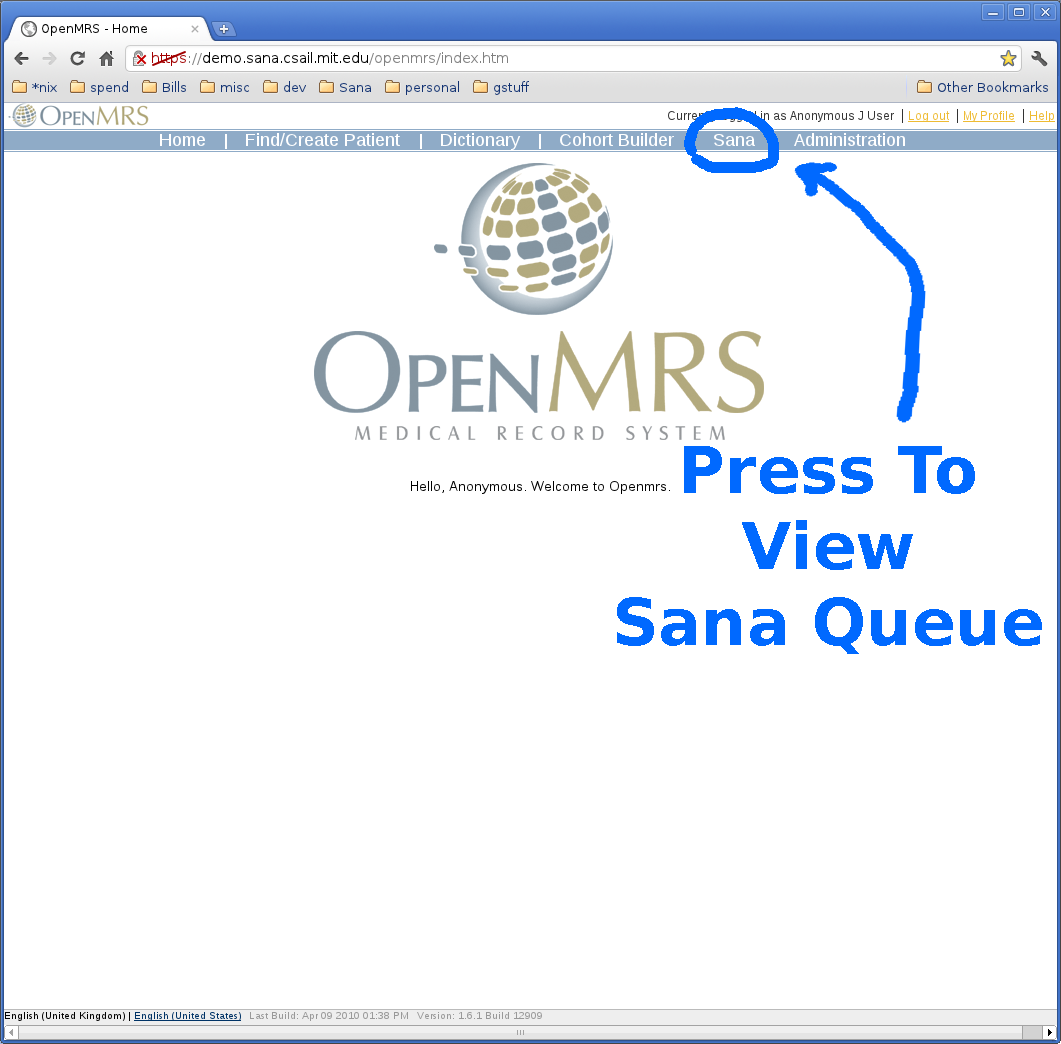
\includegraphics[scale=0.25,keepaspectratio=true]{openmrs_login_success_sana_tab.png}
\end{tabular}
\end{flushleft}

Username: guest, Password: Sanamobile1

\subsection{See the Results}
\noindent Once you have successfully logged in, your exam results will be 
visible in your browser.Click the queue of pending cases(Sana tab highlighted 
above.) Select your encounter and view it.

\begin{flushleft}
\begin{tabular}{ c c }
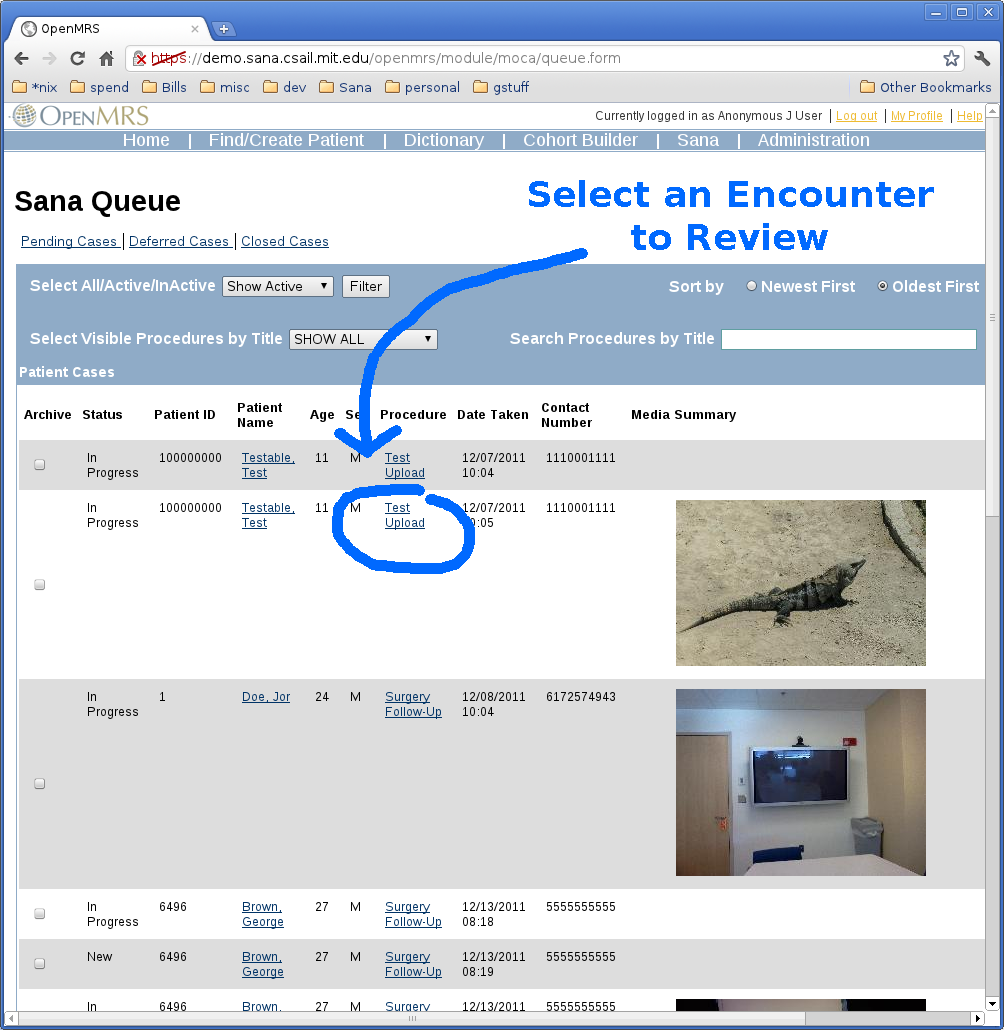
\includegraphics[scale=0.25,keepaspectratio=true]{openmrs_sana_queue.png}
&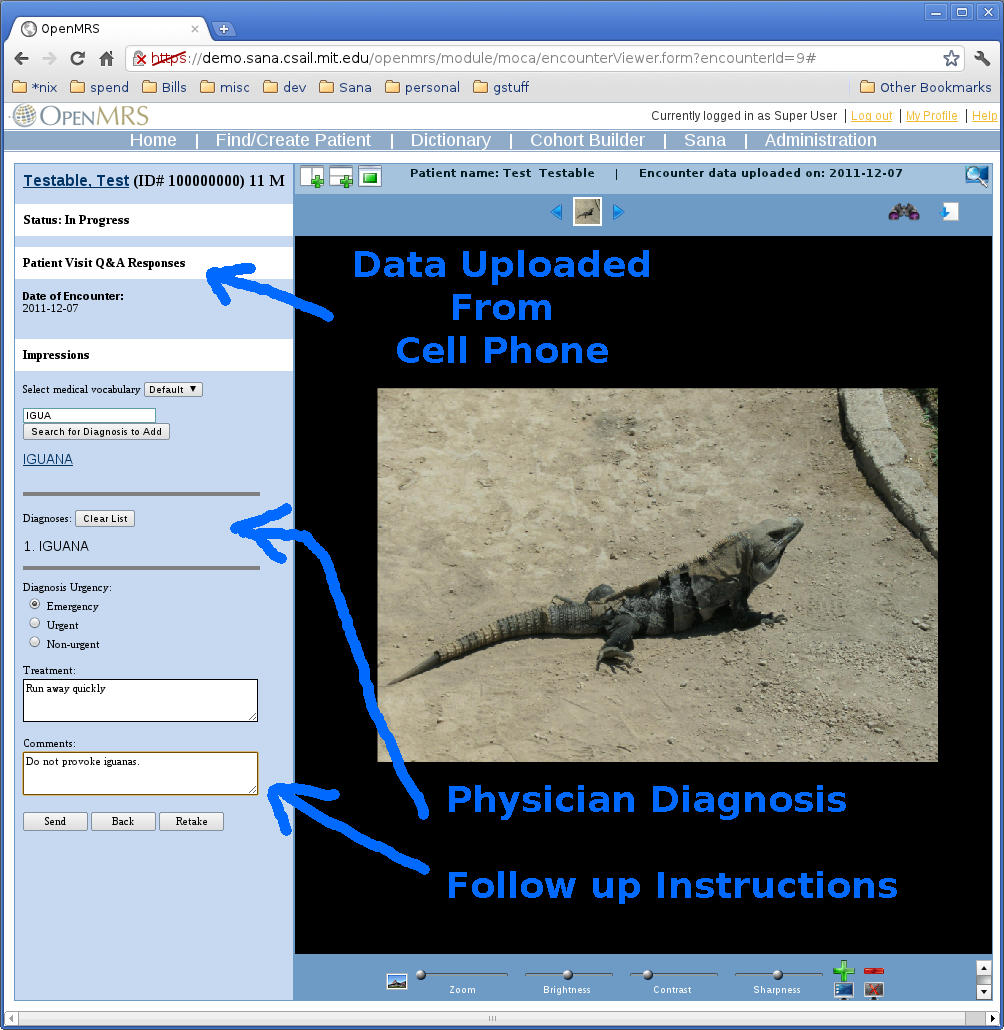
\includegraphics[scale=0.25,keepaspectratio=true]{openmrs_sana_encounter.png}
\end{tabular}
\end{flushleft}

For an actual patient encounter, reviewing clinicians would append information 
to the encounter-diagnosis, request for additional information, comments, etc.
and send a notification back to the phone

\end{document}







\clearpage{}





\clearpage{}






\section{Client User Guide: Small Scale Clinic}
Targeted at small groups (10-15) of clinicians and administrators, who want to setup a local installation of Sana. If your clinic or healthcare facility is small, and you want to use Sana to track routine changes or occurances in your paitent population (usually fewer than 100 patients), this is your guide.


\clearpage{}

\section{Glossary of Terms}

\end{document}
